% Static report, BUAN 314-370 course project, Brennan Martin.
% Compile in Overleaf with pdfLaTeX (main file: main.tex).
% No number in the text is typed by hand: every one is \V{key}, defined in numbers.tex,
% which scripts/08_report_numbers.R writes from the files in output/tables.
%
% WHOSE WORDS: the text of this report was drafted by the AI assistant (decision D-024,
% documentation/process/assistant_drafts.md). Brennan keeps or changes it at his final
% pass. While \drafttrue is set, every page says so. Set \draftfalse only after that pass.
\documentclass[11pt]{article}
\usepackage[margin=1in]{geometry}
\usepackage[T1]{fontenc}
\usepackage[utf8]{inputenc}
\usepackage{lmodern}
\usepackage{microtype}
\usepackage{graphicx}
\usepackage{booktabs}
\usepackage{longtable}
\usepackage{array}
\usepackage{caption}
\usepackage{float}
\usepackage{xcolor}
\usepackage{enumitem}
\usepackage{fancyhdr}
\usepackage[hidelinks]{hyperref}

% Written by scripts/08_report_numbers.R. Do not edit by hand.
% Every number in the report is \V{key}; the key, value and source file are listed in output/tables/report_numbers.csv.
\newcommand{\V}[1]{\ifcsname val@#1\endcsname\csname val@#1\endcsname\else\textbf{[missing number: \detokenize{#1}]}\fi}
\expandafter\def\csname val@cells_read\endcsname{1,956}
\expandafter\def\csname val@rows_after_duplicates\endcsname{1,068}
\expandafter\def\csname val@rows_duplicates_removed\endcsname{888}
\expandafter\def\csname val@rows_after_unreported\endcsname{1,038}
\expandafter\def\csname val@rows_unreported_removed\endcsname{30}
\expandafter\def\csname val@rows_after_no_wagering\endcsname{924}
\expandafter\def\csname val@rows_no_wagering_removed\endcsname{114}
\expandafter\def\csname val@rows_negative_removed\endcsname{1}
\expandafter\def\csname val@rows_final\endcsname{923}
\expandafter\def\csname val@lump_months\endcsname{21}
\expandafter\def\csname val@first_months\endcsname{15}
\expandafter\def\csname val@cleaning_steps\endcsname{18}
\expandafter\def\csname val@cleaning_decisions\endcsname{17}
\expandafter\def\csname val@fp_rows\endcsname{919}
\expandafter\def\csname val@fp_missing\endcsname{4}
\expandafter\def\csname val@fp_q1\endcsname{1.90}
\expandafter\def\csname val@fp_median\endcsname{3.71}
\expandafter\def\csname val@fp_q3\endcsname{5.53}
\expandafter\def\csname val@fp_mean\endcsname{5.18}
\expandafter\def\csname val@fp_max\endcsname{121.84}
\expandafter\def\csname val@fp_p95\endcsname{14.68}
\expandafter\def\csname val@fp_n_5plus\endcsname{277}
\expandafter\def\csname val@fp_pct_5plus\endcsname{30.14}
\expandafter\def\csname val@fp_n_10plus\endcsname{81}
\expandafter\def\csname val@fp_pct_10plus\endcsname{8.81}
\expandafter\def\csname val@fp_pct_10plus_round\endcsname{9}
\expandafter\def\csname val@fp_n_under1\endcsname{122}
\expandafter\def\csname val@fp_pct_under1\endcsname{13.28}
\expandafter\def\csname val@fp_n_3to4\endcsname{168}
\expandafter\def\csname val@fp_pct_3to4\endcsname{18.28}
\expandafter\def\csname val@fp_n_20plus\endcsname{29}
\expandafter\def\csname val@notax_n\endcsname{449}
\expandafter\def\csname val@notax_pct\endcsname{48.65}
\expandafter\def\csname val@tax_n\endcsname{474}
\expandafter\def\csname val@tax_pct\endcsname{51.35}
\expandafter\def\csname val@notax_pct_round\endcsname{49}
\expandafter\def\csname val@n_operators\endcsname{15}
\expandafter\def\csname val@n_commercial\endcsname{3}
\expandafter\def\csname val@n_tribal\endcsname{12}
\expandafter\def\csname val@share_top1\endcsname{33.48}
\expandafter\def\csname val@share_top2\endcsname{27.46}
\expandafter\def\csname val@share_top3\endcsname{16.29}
\expandafter\def\csname val@share_top3_total\endcsname{77.22}
\expandafter\def\csname val@share_top3_round\endcsname{77}
\expandafter\def\csname val@share_top6\endcsname{94.30}
\expandafter\def\csname val@share_bottom9\endcsname{5.70}
\expandafter\def\csname val@share_bottom9_round\endcsname{6}
\expandafter\def\csname val@months_full\endcsname{70}
\expandafter\def\csname val@months_fewest\endcsname{37}
\expandafter\def\csname val@total_wagered_billion\endcsname{28.0}
\expandafter\def\csname val@op_lvd_median\endcsname{6.34}
\expandafter\def\csname val@op_lvd_months\endcsname{70}
\expandafter\def\csname val@op_hannahville_median\endcsname{5.13}
\expandafter\def\csname val@op_hannahville_months\endcsname{66}
\expandafter\def\csname val@op_betmgm_median\endcsname{4.39}
\expandafter\def\csname val@op_betmgm_months\endcsname{70}
\expandafter\def\csname val@op_fanduel_median\endcsname{3.83}
\expandafter\def\csname val@op_fanduel_months\endcsname{70}
\expandafter\def\csname val@op_draftkings_median\endcsname{3.54}
\expandafter\def\csname val@op_draftkings_months\endcsname{70}
\expandafter\def\csname val@op_pokagon_median\endcsname{0.46}
\expandafter\def\csname val@op_pokagon_months\endcsname{67}
\expandafter\def\csname val@op_sault_median\endcsname{0.83}
\expandafter\def\csname val@op_sault_months\endcsname{39}
\expandafter\def\csname val@op_pokagon_q1\endcsname{0.05}
\expandafter\def\csname val@op_pokagon_q3\endcsname{11.35}
\expandafter\def\csname val@op_fanduel_rank\endcsname{6}
\expandafter\def\csname val@op_draftkings_rank\endcsname{8}
\expandafter\def\csname val@yr_2021_median\endcsname{5.79}
\expandafter\def\csname val@yr_2021_months\endcsname{154}
\expandafter\def\csname val@yr_2022_median\endcsname{4.04}
\expandafter\def\csname val@yr_2022_months\endcsname{175}
\expandafter\def\csname val@yr_2023_median\endcsname{3.39}
\expandafter\def\csname val@yr_2023_months\endcsname{175}
\expandafter\def\csname val@yr_2024_median\endcsname{3.56}
\expandafter\def\csname val@yr_2024_months\endcsname{148}
\expandafter\def\csname val@yr_2025_median\endcsname{3.02}
\expandafter\def\csname val@yr_2025_months\endcsname{140}
\expandafter\def\csname val@yr_2026_median\endcsname{3.09}
\expandafter\def\csname val@yr_2026_months\endcsname{127}
\expandafter\def\csname val@com_median\endcsname{3.88}
\expandafter\def\csname val@com_months\endcsname{210}
\expandafter\def\csname val@com_rows\endcsname{210}
\expandafter\def\csname val@com_q1\endcsname{2.90}
\expandafter\def\csname val@com_q3\endcsname{4.70}
\expandafter\def\csname val@com_mean\endcsname{4.73}
\expandafter\def\csname val@tri_median\endcsname{3.65}
\expandafter\def\csname val@tri_months\endcsname{709}
\expandafter\def\csname val@tri_rows\endcsname{713}
\expandafter\def\csname val@tri_q1\endcsname{1.60}
\expandafter\def\csname val@tri_q3\endcsname{6.15}
\expandafter\def\csname val@tri_mean\endcsname{5.32}
\expandafter\def\csname val@r_fp_size\endcsname{-0.07}
\expandafter\def\csname val@rank_fp_size\endcsname{0.12}
\expandafter\def\csname val@size_band1_median\endcsname{2.27}
\expandafter\def\csname val@size_band1_months\endcsname{146}
\expandafter\def\csname val@size_band2_median\endcsname{3.67}
\expandafter\def\csname val@size_band2_months\endcsname{349}
\expandafter\def\csname val@size_band3_median\endcsname{3.89}
\expandafter\def\csname val@size_band3_months\endcsname{324}
\expandafter\def\csname val@size_band4_median\endcsname{3.88}
\expandafter\def\csname val@size_band4_months\endcsname{100}
\expandafter\def\csname val@size_band1_mean\endcsname{7.18}
\expandafter\def\csname val@com_notax_n\endcsname{45}
\expandafter\def\csname val@com_notax_pct\endcsname{21.43}
\expandafter\def\csname val@tri_notax_n\endcsname{404}
\expandafter\def\csname val@tri_notax_pct\endcsname{56.66}
\expandafter\def\csname val@com_2021_notax_pct\endcsname{16.67}
\expandafter\def\csname val@com_2021_notax_round\endcsname{17}
\expandafter\def\csname val@com_2021_notax_n\endcsname{6}
\expandafter\def\csname val@com_2021_rows\endcsname{36}
\expandafter\def\csname val@tri_2021_notax_pct\endcsname{73.95}
\expandafter\def\csname val@tri_2021_notax_round\endcsname{74}
\expandafter\def\csname val@tri_2021_notax_n\endcsname{88}
\expandafter\def\csname val@tri_2021_rows\endcsname{119}
\expandafter\def\csname val@com_2022_notax_pct\endcsname{0.00}
\expandafter\def\csname val@com_2022_notax_round\endcsname{0}
\expandafter\def\csname val@com_2022_notax_n\endcsname{0}
\expandafter\def\csname val@com_2022_rows\endcsname{36}
\expandafter\def\csname val@tri_2022_notax_pct\endcsname{69.50}
\expandafter\def\csname val@tri_2022_notax_round\endcsname{70}
\expandafter\def\csname val@tri_2022_notax_n\endcsname{98}
\expandafter\def\csname val@tri_2022_rows\endcsname{141}
\expandafter\def\csname val@com_2023_notax_pct\endcsname{11.11}
\expandafter\def\csname val@com_2023_notax_round\endcsname{11}
\expandafter\def\csname val@com_2023_notax_n\endcsname{4}
\expandafter\def\csname val@com_2023_rows\endcsname{36}
\expandafter\def\csname val@tri_2023_notax_pct\endcsname{54.68}
\expandafter\def\csname val@tri_2023_notax_round\endcsname{55}
\expandafter\def\csname val@tri_2023_notax_n\endcsname{76}
\expandafter\def\csname val@tri_2023_rows\endcsname{139}
\expandafter\def\csname val@com_2024_notax_pct\endcsname{55.56}
\expandafter\def\csname val@com_2024_notax_round\endcsname{56}
\expandafter\def\csname val@com_2024_notax_n\endcsname{20}
\expandafter\def\csname val@com_2024_rows\endcsname{36}
\expandafter\def\csname val@tri_2024_notax_pct\endcsname{69.03}
\expandafter\def\csname val@tri_2024_notax_round\endcsname{69}
\expandafter\def\csname val@tri_2024_notax_n\endcsname{78}
\expandafter\def\csname val@tri_2024_rows\endcsname{113}
\expandafter\def\csname val@com_2025_notax_pct\endcsname{41.67}
\expandafter\def\csname val@com_2025_notax_round\endcsname{42}
\expandafter\def\csname val@com_2025_notax_n\endcsname{15}
\expandafter\def\csname val@com_2025_rows\endcsname{36}
\expandafter\def\csname val@tri_2025_notax_pct\endcsname{43.27}
\expandafter\def\csname val@tri_2025_notax_round\endcsname{43}
\expandafter\def\csname val@tri_2025_notax_n\endcsname{45}
\expandafter\def\csname val@tri_2025_rows\endcsname{104}
\expandafter\def\csname val@com_2026_notax_pct\endcsname{0.00}
\expandafter\def\csname val@com_2026_notax_round\endcsname{0}
\expandafter\def\csname val@com_2026_notax_n\endcsname{0}
\expandafter\def\csname val@com_2026_rows\endcsname{30}
\expandafter\def\csname val@tri_2026_notax_pct\endcsname{19.59}
\expandafter\def\csname val@tri_2026_notax_round\endcsname{20}
\expandafter\def\csname val@tri_2026_notax_n\endcsname{19}
\expandafter\def\csname val@tri_2026_rows\endcsname{97}
\expandafter\def\csname val@age_com_b1_median\endcsname{3.43}
\expandafter\def\csname val@age_com_b1_months\endcsname{18}
\expandafter\def\csname val@age_com_b2_median\endcsname{3.74}
\expandafter\def\csname val@age_com_b2_months\endcsname{18}
\expandafter\def\csname val@age_com_b3_median\endcsname{3.36}
\expandafter\def\csname val@age_com_b3_months\endcsname{36}
\expandafter\def\csname val@age_com_b4_median\endcsname{3.76}
\expandafter\def\csname val@age_com_b4_months\endcsname{72}
\expandafter\def\csname val@age_com_b5_median\endcsname{4.15}
\expandafter\def\csname val@age_com_b5_months\endcsname{66}
\expandafter\def\csname val@age_tri_b1_median\endcsname{9.05}
\expandafter\def\csname val@age_tri_b1_months\endcsname{71}
\expandafter\def\csname val@age_tri_b2_median\endcsname{6.14}
\expandafter\def\csname val@age_tri_b2_months\endcsname{72}
\expandafter\def\csname val@age_tri_b3_median\endcsname{3.97}
\expandafter\def\csname val@age_tri_b3_months\endcsname{142}
\expandafter\def\csname val@age_tri_b4_median\endcsname{2.78}
\expandafter\def\csname val@age_tri_b4_months\endcsname{258}
\expandafter\def\csname val@age_tri_b5_median\endcsname{2.52}
\expandafter\def\csname val@age_tri_b5_months\endcsname{166}
\expandafter\def\csname val@age_com_min\endcsname{3.36}
\expandafter\def\csname val@age_com_max\endcsname{4.15}
\expandafter\def\csname val@without_median\endcsname{3.65}
\expandafter\def\csname val@without_months\endcsname{888}
\expandafter\def\csname val@without_mean\endcsname{4.17}
\expandafter\def\csname val@without_2021\endcsname{4.66}
\expandafter\def\csname val@without_2026\endcsname{3.03}
\expandafter\def\csname val@without_pct_5plus\endcsname{27.70}
\expandafter\def\csname val@without_lump_mean\endcsname{4.31}
\expandafter\def\csname val@without_lump_median\endcsname{3.67}
\expandafter\def\csname val@lump_2021\endcsname{15}
\expandafter\def\csname val@first_2021\endcsname{14}
\expandafter\def\csname val@r_fp_prior\endcsname{0.59}
\expandafter\def\csname val@r_fp_prior_rows\endcsname{900}
\expandafter\def\csname val@r_fp_months\endcsname{-0.26}
\expandafter\def\csname val@r_fp_lump\endcsname{0.76}
\expandafter\def\csname val@r_fp_commercial\endcsname{-0.03}
\expandafter\def\csname val@r_nt_prior\endcsname{0.79}
\expandafter\def\csname val@r_nt_prior_rows\endcsname{906}
\expandafter\def\csname val@r_nt_priorsize\endcsname{-0.46}
\expandafter\def\csname val@r_nt_commercial\endcsname{-0.30}
\expandafter\def\csname val@r_nt_months\endcsname{-0.28}
\expandafter\def\csname val@r_nt_fp\endcsname{0.23}
\expandafter\def\csname val@m1_b0\endcsname{3.2356}
\expandafter\def\csname val@m1_b0_se\endcsname{0.4271}
\expandafter\def\csname val@m1_b0_p\endcsname{under 0.001}
\expandafter\def\csname val@m1_b1\endcsname{0.4975}
\expandafter\def\csname val@m1_b1_se\endcsname{0.0243}
\expandafter\def\csname val@m1_b1_p\endcsname{under 0.001}
\expandafter\def\csname val@m1_b2\endcsname{0.0323}
\expandafter\def\csname val@m1_b2_se\endcsname{0.0099}
\expandafter\def\csname val@m1_b2_p\endcsname{0.001}
\expandafter\def\csname val@m1_b3\endcsname{0.1308}
\expandafter\def\csname val@m1_b3_se\endcsname{0.4354}
\expandafter\def\csname val@m1_b3_p\endcsname{0.76}
\expandafter\def\csname val@m2_b0\endcsname{0.6532}
\expandafter\def\csname val@m2_b0_se\endcsname{0.1085}
\expandafter\def\csname val@m2_b0_p\endcsname{under 0.001}
\expandafter\def\csname val@m2_b1\endcsname{0.7353}
\expandafter\def\csname val@m2_b1_se\endcsname{0.0222}
\expandafter\def\csname val@m2_b1_p\endcsname{under 0.001}
\expandafter\def\csname val@m2_b2\endcsname{0.0771}
\expandafter\def\csname val@m2_b2_se\endcsname{0.0156}
\expandafter\def\csname val@m2_b2_p\endcsname{under 0.001}
\expandafter\def\csname val@m2_b3\endcsname{0.0084}
\expandafter\def\csname val@m2_b3_se\endcsname{0.0289}
\expandafter\def\csname val@m2_b3_p\endcsname{0.77}
\expandafter\def\csname val@m1_prior_cents\endcsname{50}
\expandafter\def\csname val@m1_months_cents\endcsname{3}
\expandafter\def\csname val@m1_months_year\endcsname{0.39}
\expandafter\def\csname val@m1_com_dollars\endcsname{0.13}
\expandafter\def\csname val@m1_com_se_dollars\endcsname{0.44}
\expandafter\def\csname val@m2_prior_points\endcsname{73.5}
\expandafter\def\csname val@m2_size_points\endcsname{7.7}
\expandafter\def\csname val@m2_com_points\endcsname{0.8}
\expandafter\def\csname val@m2_com_se_points\endcsname{2.9}
\expandafter\def\csname val@m1_rows\endcsname{900}
\expandafter\def\csname val@m1_left_out\endcsname{23}
\expandafter\def\csname val@m1_r2\endcsname{0.357}
\expandafter\def\csname val@m1_r2_pct\endcsname{35.7}
\expandafter\def\csname val@m1_r2_round\endcsname{36}
\expandafter\def\csname val@m1_rmse\endcsname{5.46}
\expandafter\def\csname val@m2_rows\endcsname{906}
\expandafter\def\csname val@m2_left_out\endcsname{17}
\expandafter\def\csname val@m2_r2\endcsname{0.645}
\expandafter\def\csname val@m2_min\endcsname{-0.0023}
\expandafter\def\csname val@m2_max\endcsname{1.171}
\expandafter\def\csname val@m2_below0\endcsname{3}
\expandafter\def\csname val@m2_above1\endcsname{2}
\expandafter\def\csname val@m2_outside\endcsname{5}
\expandafter\def\csname val@m2_outside_pct\endcsname{0.55}
\expandafter\def\csname val@m2_correct_pct\endcsname{89.7}
\expandafter\def\csname val@m2_correct_round\endcsname{90}
\expandafter\def\csname val@m2_baseline_pct\endcsname{51.8}
\expandafter\def\csname val@m2_baseline_round\endcsname{52}
\expandafter\def\csname val@m2_share_yes\endcsname{48.2}
\expandafter\def\csname val@m2_mean_pred\endcsname{48.2}
\expandafter\def\csname val@m2_yes_yes\endcsname{394}
\expandafter\def\csname val@m2_yes_no\endcsname{43}
\expandafter\def\csname val@m2_no_yes\endcsname{50}
\expandafter\def\csname val@m2_no_no\endcsname{419}
\expandafter\def\csname val@m2_correct_n\endcsname{813}
\expandafter\def\csname val@m2_actual_yes\endcsname{437}
\expandafter\def\csname val@m2_actual_no\endcsname{469}
\expandafter\def\csname val@m1_within5_n\endcsname{846}
\expandafter\def\csname val@m1_within5_pct\endcsname{94}
\expandafter\def\csname val@m1_above10\endcsname{18}
\expandafter\def\csname val@m1_below10\endcsname{2}
\expandafter\def\csname val@m1_largest_miss\endcsname{118.56}
\expandafter\def\csname val@m1_above10_lump\endcsname{12}
\expandafter\def\csname val@m1_no_prior\endcsname{17}
\expandafter\def\csname val@m1_missing_value\endcsname{6}
\expandafter\def\csname val@m2_no_prior\endcsname{17}
\expandafter\def\csname val@case1_m1\endcsname{3.81}
\expandafter\def\csname val@case1_m2\endcsname{0.0278}
\expandafter\def\csname val@case1_m2_pct\endcsname{3}
\expandafter\def\csname val@case2_m1\endcsname{3.78}
\expandafter\def\csname val@case2_m2\endcsname{0.9122}
\expandafter\def\csname val@case2_m2_pct\endcsname{91}
\expandafter\def\csname val@case3_m1\endcsname{7.58}
\expandafter\def\csname val@case3_m2\endcsname{0.8889}
\expandafter\def\csname val@case3_m2_pct\endcsname{89}
\expandafter\def\csname val@hand_checks\endcsname{6}
\expandafter\def\csname val@hand_equal\endcsname{6}
\expandafter\def\csname val@tests_run\endcsname{11}
\expandafter\def\csname val@figure_checks\endcsname{15}
\expandafter\def\csname val@def_cutoff\endcsname{0.5}
\expandafter\def\csname val@def_per\endcsname{100}
\expandafter\def\csname val@def_lump_share\endcsname{a quarter}
\expandafter\def\csname val@def_tiny_handle\endcsname{10,000}
\expandafter\def\csname val@def_small_group\endcsname{30}
\expandafter\def\csname val@def_within\endcsname{5}
\expandafter\def\csname val@def_fp_mid\endcsname{5}
\expandafter\def\csname val@def_fp_high\endcsname{10}
\expandafter\def\csname val@def_frame\endcsname{20}
\expandafter\def\csname val@def_big_miss\endcsname{10}
\expandafter\def\csname val@n_columns\endcsname{28}
\expandafter\def\csname val@tax_rate\endcsname{8.4}
\expandafter\def\csname val@tax_rate_state_commercial\endcsname{5.88}


\newif\ifdraft
\drafttrue

\newcommand{\repo}{https://github.com/BrennanKM/buan314-370-project-martin}
\newcommand{\pageaddress}{https://brennankm.github.io/buan314-370-project-martin/}

\captionsetup{font=small,labelfont=bf}
\setlength{\parskip}{0.5em}
\setlength{\parindent}{0pt}
\setlist{itemsep=0.2em,topsep=0.3em}
\renewcommand{\arraystretch}{1.15}

\pagestyle{fancy}
\fancyhf{}
\renewcommand{\headrulewidth}{0pt}
\fancyfoot[C]{\thepage}
\ifdraft
  \fancyhead[C]{\small\color{gray}Draft: text written by the AI assistant, not yet revised by Brennan Martin}
\fi

\begin{document}

\begin{titlepage}
\thispagestyle{empty}
\vspace*{2cm}
{\LARGE\bfseries Free play and tax in Michigan's online sports betting market\par}
\vspace{0.6cm}
{\large How much free play sportsbooks deduct, and how often a sportsbook pays no state tax, January 2021 to October 2026\par}
\vspace{1.4cm}
{\large Brennan Martin\par}
\vspace{0.3cm}
BUAN 314-370, Descriptive Analytics and Data Management\\
University of San Diego, Fall 2026\\
Dr. Steven Levkoff\par
\vspace{0.3cm}
% Date of the final version goes here when the report is final.
Draft of 24 November 2026\par
\vspace{1.4cm}
\begin{tabular}{@{}ll@{}}
Repository: & \url{\repo} \\
Interactive report: & \url{\pageaddress} \\
Recorded presentation: & link to be added when the talk is recorded \\
\end{tabular}
\ifdraft
\vfill
\fbox{\parbox{0.92\linewidth}{\small\textbf{Draft.} The numbers, tables and figures in this report are produced by the project's scripts. The wording of the text was drafted by the AI assistant and has not yet been revised by Brennan Martin. This notice is removed only after his revision.}}
\fi
\end{titlepage}

\section*{Executive summary}
\addcontentsline{toc}{section}{Executive summary}

Michigan lets online sportsbooks subtract the free bets they hand out before tax is figured. This report, written for the Michigan Gaming Control Board, asks how much they subtract and how often a sportsbook pays the State nothing in a month.

The data are the Board's monthly figures for all \V{n_operators} licensed operators, January 2021 to October 2026: \V{rows_final} sportsbook-months.

First, the typical month deducts \$\V{fp_median} of free play per \$100 wagered; half of all months fall between \$\V{fp_q1} and \$\V{fp_q3}, and \V{fp_pct_10plus}\% reach \$\V{def_fp_high} or more. Second, no state tax was paid in \V{notax_pct}\% of sportsbook-months. For tribal operators that share fell from \V{tri_2021_notax_round}\% in 2021 to \V{tri_2026_notax_round}\% in 2026. Third, heavy free play belongs to the early months of tribal sportsbooks (\$\V{age_tri_b1_median} per \$100 in their first six months, \$\V{age_tri_b5_median} after four years); the three biggest brands, with \V{share_top3_round}\% of all dollars wagered, sit near the median.

Two linear regressions use only what is known at the start of a month. The first predicts free play per \$100 with a typical miss of \$\V{m1_rmse}, too wide to rely on. The second calls whether a sportsbook will pay no tax correctly in \V{m2_correct_pct}\% of months, against \V{m2_baseline_pct}\% for always guessing the more common outcome. Both were judged on the months they were fitted to.

Recommendation: review first the claims of small sportsbooks that paid no tax last month, track lump deductions separately, and collect free play issued by month before studying any cap.

\section{Business problem}

\subsection*{The setting}
Internet sports betting began in Michigan on 22 January 2021 \cite{mgcb_data}. Each licensed operator reports to the Michigan Gaming Control Board every month \cite{mcl_416a}. Tax is not charged on everything a sportsbook wins from bettors. The law lets an operator first subtract the value of the free play its customers wagered \cite{mcl_403}, and the tax or payment to the State is \V{tax_rate}\% of what is left. A sportsbook that gives away enough free bets in a month can therefore owe nothing.

Free play is also a promotion: it gives a bettor something to wager that is not the bettor's own money. A regulator that wants to protect bettors and the State's revenue has a reason to know how large the deduction is, who uses it most, and whether it is shrinking as the market gets older.

\subsection*{The decision-maker}
The Michigan Gaming Control Board, which receives the operators' monthly reports and publishes them.

\subsection*{The three problem statements}
\begin{description}[leftmargin=1.2em,style=nextline]
\item[Descriptive] The Michigan Gaming Control Board needs to see how much free play the state's online sportsbooks deducted for every \$100 wagered, and how often a sportsbook paid no state tax in a month, across the \V{n_operators} licensed operators, commercial and tribal, month by month from January 2021 to October 2026, to learn which sportsbooks lean hardest on free-bet promotions and whether that reliance is fading.
\item[Predictive] At the start of each month, using only what each sportsbook reported in earlier months, the Board wants two estimates for that sportsbook's month ahead: the free play it will deduct per \$100 wagered (a percent), and whether it will pay no state tax that month (yes or no), so that staff can review the free-play claims of the flagged sportsbooks first.
\item[Prescriptive] Given those estimates, what cap on the monthly free-play deduction, as a percent of a sportsbook's gross sports betting receipts, should the Board recommend that the Legislature write into law, to collect the most state and city tax, with one cap for every operator and no cap below the share of gross receipts that the median sportsbook-month actually deducted?
\end{description}

This report takes up the first two. Sections~\ref{sec:data} to \ref{sec:eda} answer the descriptive statement. Section~\ref{sec:models} makes a first pass at the predictive one, with a linear regression for the numeric target and a linear probability model for the yes-or-no target. The prescriptive statement is not solved here; Section~\ref{sec:next} says what it would need.

\section{Data}\label{sec:data}

The data are the Michigan Gaming Control Board's ``Internet Sports Betting Revenues and Taxes'' workbooks, one for each year from 2021 to 2026 \cite{mgcb_data}. The Board is the primary source: the figures are the ones operators file with it under the Lawful Sports Betting Act. I downloaded the six workbooks by hand on 23 November 2026, because the State's site terms do not allow automated access \cite{migov_terms}. The same terms do not allow the files to be republished, so the repository holds the download steps and a checksum for each file in place of the files themselves. A script compares the files with those checksums before anything else runs.

One row is one licensed operator in one month. The data cover every operator licensed for internet sports betting in Michigan: \V{n_commercial} commercial Detroit casinos and \V{n_tribal} tribal operators, each working with a platform brand such as FanDuel or DraftKings. The period is January 2021 to October 2026. After cleaning there are \V{rows_final} rows and \V{n_columns} columns. Retail betting inside casinos and internet casino games are not in these files.

The publisher gives four dollar amounts for each operator and month. The other variables in Table~\ref{tab:variables} were built from them. The full codebook is in Appendix~A.

\begin{table}[H]
\centering\small
\caption{Key variables. Source: codebook (Appendix A).}\label{tab:variables}
% Written by scripts/08_report_numbers.R from output/tables. Do not edit by hand.
\begin{tabular}{@{}p{0.24\linewidth}p{0.50\linewidth}p{0.20\linewidth}@{}}
\toprule
Variable & What it is & Units \\
\midrule
operator & Licensed internet sports betting operator (the licensee) & none \\
operator\_type & Whether the operator is a commercial Detroit casino or a tribal operator & none \\
month\_date & First day of the reporting month & date \\
handle & Total dollars wagered online with the operator in the month & US dollars \\
gross\_receipts & Gross sports betting receipts: all sums wagered with the operator, less winnings, refunded or voided wagers, and uncollectible amounts & US dollars \\
adjusted\_gross\_receipts & Adjusted gross sports betting receipts: gross receipts less the deduction for free play & US dollars \\
state\_tax\_or\_payment & Tax (commercial operators) or payment (tribal operators) to the State for the month, as reported & US dollars \\
free\_play\_per\_100 & Free play deducted per \$100 wagered & dollars per \$100 wagered (percent of handle) \\
paid\_no\_tax & Whether the operator paid no state tax or payment for the month & none \\
months\_active & Count of months with wagering for this operator up to and including this one & months \\
lump\_deduction & Whether the free play deducted is more than a quarter of the month's handle & none \\
first\_active\_month & Whether this is the operator's first month with wagering & none \\
\bottomrule
\end{tabular}

\end{table}

Two points about measurement matter for everything that follows. The files have no free-play column. Free play is taken as gross receipts minus adjusted gross receipts, which the law defines as the free-play deduction \cite{mcl_403}; it is the amount claimed for tax in that month, and an operator can claim it later than the promotion. And the publisher does not define ``Total Handle''; this report reads it as total dollars wagered.

\section{Preparing the data}

Every cleaning step was proposed with at least two options, decided by me, carried out by a numbered script and logged with its row count. Table~\ref{tab:rows} shows the steps that changed the number of rows. The full log of \V{cleaning_steps} entries is in Appendix~B.

\begin{table}[H]
\centering\small
\caption{Row accounting. Source: wrangling log (Appendix B).}\label{tab:rows}
% Written by scripts/08_report_numbers.R from output/tables. Do not edit by hand.
\begin{tabular}{@{}p{0.07\linewidth}p{0.61\linewidth}rr@{}}
\toprule
Step & What was done & Rows before & Rows after \\
\midrule
1 & Reshaped the wide workbooks to one row per operator per month. No value changed. & 1,956 & 1,956 \\
2 & Kept each year's copy from the newest workbook that carries it; removed the duplicate copy. & 1,956 & 1,068 \\
3 & Dropped months that are blank for every operator & 1,068 & 1,038 \\
4 & Dropped operator-months with no wagering: Total Handle zero & 1,038 & 924 \\
5 & Dropped the row with a negative Total Handle & 924 & 923 \\
\bottomrule
\end{tabular}

\end{table}

The workbooks are laid out sideways, four columns per operator, so the first step turned them into one row per operator per month: \V{cells_read} rows, with no value changed. Every year but the last appears in two workbooks and the copies agree, so one copy was kept, removing \V{rows_duplicates_removed} duplicates. \V{rows_unreported_removed} rows for two months not yet reported were dropped. So were \V{rows_no_wagering_removed} months in which an operator took no wagers, because the question is about sportsbooks that are operating and those rows would each count as a month with no tax. One row with a negative amount wagered, a closing correction after an operator stopped, was dropped. That leaves \V{rows_final}: \V{cells_read} $-$ \V{rows_duplicates_removed} $-$ \V{rows_unreported_removed} $-$ \V{rows_no_wagering_removed} $-$ \V{rows_negative_removed} $=$ \V{rows_final}.

No row was removed for having an extreme value, and no missing value was filled in. Three choices keep unusual months in the data but visible:

\begin{itemize}
\item Free play per \$100 is left blank in \V{fp_missing} months: two with under \$\V{def_tiny_handle} wagered, where a ratio means little, and two where the reported deduction is negative.
\item \V{lump_months} months in which the deduction is more than \V{def_lump_share} of the dollars wagered are flagged as lump deductions. They look like free play claimed late in one piece. The largest is \$\V{fp_max} per \$100, in a month for which the Board's own release reports a deduction that had not been taken earlier \cite{mgcb_release_2024}.
\item Each operator's first month with wagering, \V{first_months} in all, is flagged because it is a partial month.
\end{itemize}

Section~\ref{sec:eda} reports how much the flagged months move the results. A validation script runs \V{tests_run} tests on the cleaned file each time, and all pass.

\section{Exploratory analysis}\label{sec:eda}

The descriptive statement was broken into twelve sub-questions. Before any table was computed, I recorded what I expected for each one. This section goes through them in order and ends with the correlation matrix.

\subsection*{How much free play is deducted? (sub-questions 1 and 2)}

Across the \V{fp_rows} months with a value, the median sportsbook-month deducted \$\V{fp_median} of free play for every \$100 wagered. Figure~\ref{fig:spread} shows one main bunch with a long tail: half of all months fall between \$\V{fp_q1} and \$\V{fp_q3}, while \V{fp_n_10plus} months (\V{fp_pct_10plus}\%) reach \$\V{def_fp_high} or more and the largest is \$\V{fp_max}. I expected two clusters. The only sign of a second group is \V{fp_n_under1} months (\V{fp_pct_under1}\%) under \$1.

\begin{figure}[H]
\centering
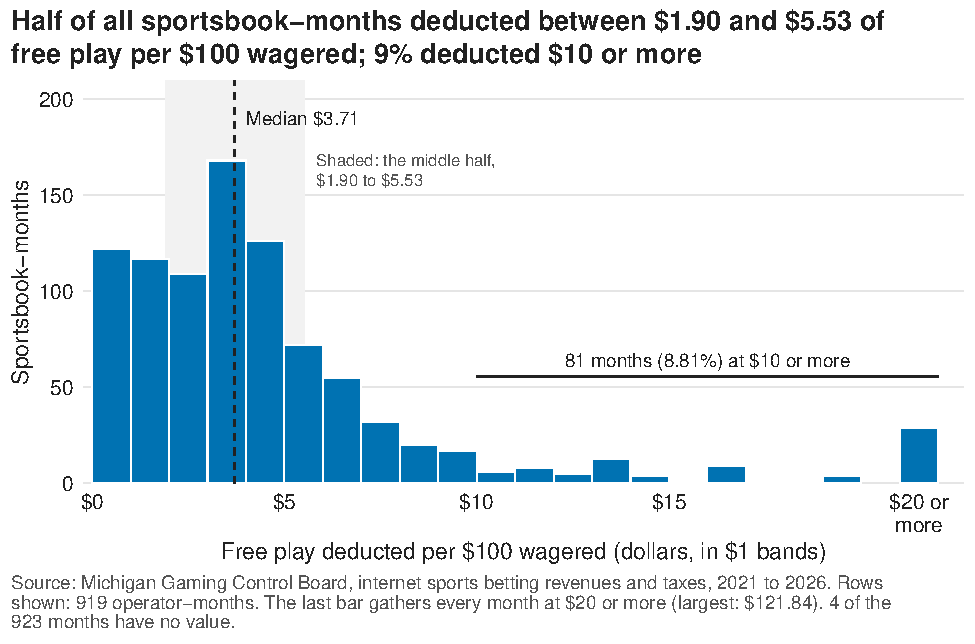
\includegraphics[width=0.92\linewidth]{figures/fig01_free_play_spread.pdf}
\caption{Spread of free play deducted per \$100 wagered (sub-question 1). Source: Michigan Gaming Control Board; \V{fp_rows} sportsbook-months.}\label{fig:spread}
\end{figure}

No state tax or payment was made in \V{notax_n} of the \V{rows_final} sportsbook-months (\V{notax_pct}\%), almost as many as the \V{tax_n} months (\V{tax_pct}\%) in which something was paid. Asked what I would have guessed before seeing any number, I said under 10\%.

\subsection*{Who are the sportsbooks, and which deduct the most? (sub-questions 3 and 4)}

The market is concentrated. Figure~\ref{fig:share} shows that three sportsbooks took \V{share_top3_total}\% of all dollars wagered: FanDuel (\V{share_top1}\%), DraftKings (\V{share_top2}\%) and BetMGM (\V{share_top3}\%). The nine smallest of the \V{n_operators} took \V{share_bottom9}\% together. I expected the top three to hold 50\% to 70\%.

\begin{figure}[H]
\centering
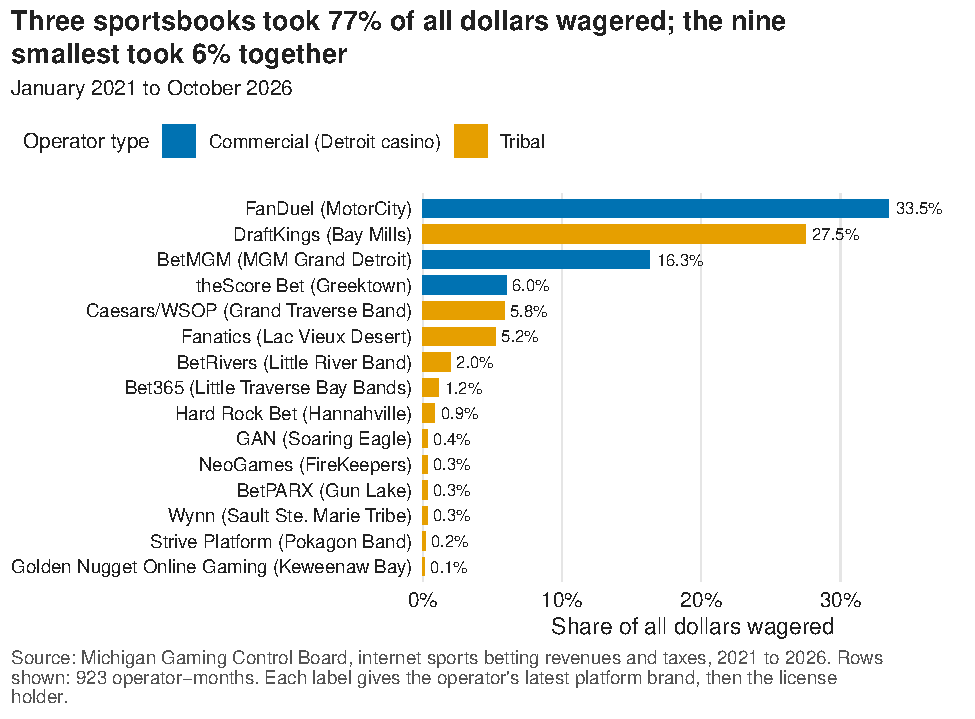
\includegraphics[width=0.92\linewidth]{figures/fig03_share_of_wagering.pdf}
\caption{Share of all dollars wagered by operator, colored by operator type (sub-question 3). Source: Michigan Gaming Control Board; \V{rows_final} sportsbook-months.}\label{fig:share}
\end{figure}

The biggest brands are not the heaviest users of free play per \$100. In Figure~\ref{fig:operators} the two highest medians belong to smaller tribal sportsbooks: Lac Vieux Desert (Fanatics) at \$\V{op_lvd_median} over \V{op_lvd_months} months and Hannahville (Hard Rock Bet) at \$\V{op_hannahville_median} over \V{op_hannahville_months}. BetMGM is third at \$\V{op_betmgm_median}. FanDuel (\$\V{op_fanduel_median}) and DraftKings (\$\V{op_draftkings_median}) sit beside the overall median of \$\V{fp_median}. The lowest median is Pokagon Band's \$\V{op_pokagon_median}, but its middle half runs from \$\V{op_pokagon_q1} to \$\V{op_pokagon_q3}, so a small sportsbook's months swing widely. I expected the big brands to deduct more. Table~\ref{tab:operators} gives the numbers behind both figures.

\begin{figure}[H]
\centering
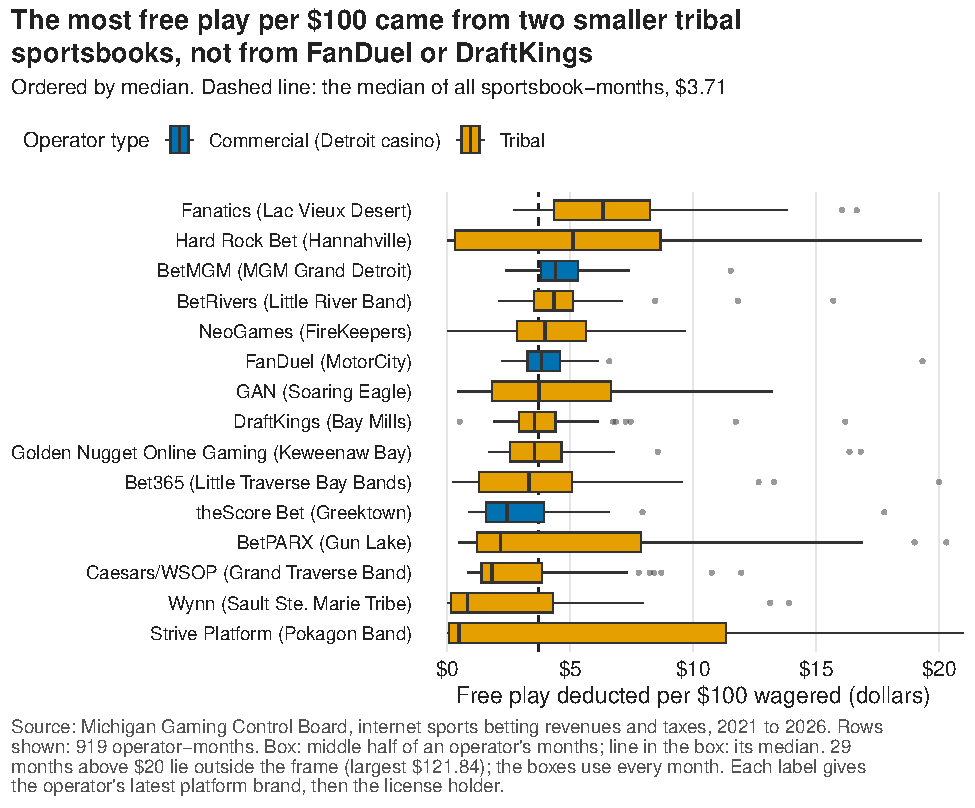
\includegraphics[width=0.92\linewidth]{figures/fig04_free_play_by_operator.pdf}
\caption{Free play deducted per \$100 wagered by operator, ordered by median (sub-question 4). \V{fp_n_20plus} months above \$\V{def_frame} are outside the frame. Source: Michigan Gaming Control Board; \V{fp_rows} sportsbook-months.}\label{fig:operators}
\end{figure}

\begin{table}[H]
\centering\footnotesize
\caption{Free play per \$100 wagered and share of all dollars wagered, by operator. Source: output/tables/eda\_03 and eda\_04.}\label{tab:operators}
% Written by scripts/08_report_numbers.R from output/tables. Do not edit by hand.
\begin{tabular}{@{}p{0.21\linewidth}p{0.20\linewidth}lrrrrr@{}}
\toprule
Operator & Brand & Type & Months & Lower quartile & Median & Upper quartile & Share of wagering (\%) \\
\midrule
Lac Vieux Desert & Fanatics & tribal & 70 & 4.34 & 6.34 & 8.25 & 5.23 \\
Hannahville & Hard Rock Bet & tribal & 66 & 0.31 & 5.13 & 8.67 & 0.87 \\
MGM Grand Detroit & BetMGM & commercial & 70 & 3.82 & 4.39 & 5.32 & 16.29 \\
Little River Band & BetRivers & tribal & 70 & 3.54 & 4.34 & 5.11 & 2.00 \\
FireKeepers & NeoGames & tribal & 64 & 2.83 & 3.96 & 5.63 & 0.34 \\
MotorCity & FanDuel & commercial & 70 & 3.26 & 3.83 & 4.57 & 33.48 \\
Soaring Eagle & GAN & tribal & 55 & 1.82 & 3.73 & 6.65 & 0.35 \\
Bay Mills & DraftKings & tribal & 70 & 2.91 & 3.54 & 4.39 & 27.46 \\
Keweenaw Bay & Golden Nugget Online Gaming & tribal & 37 & 2.54 & 3.54 & 4.64 & 0.13 \\
Little Traverse Bay Bands & Bet365 & tribal & 38 & 1.29 & 3.32 & 5.06 & 1.16 \\
Greektown & theScore Bet & commercial & 70 & 1.57 & 2.43 & 3.92 & 5.99 \\
Gun Lake & BetPARX & tribal & 63 & 1.20 & 2.16 & 7.87 & 0.33 \\
Grand Traverse Band & Caesars/WSOP & tribal & 70 & 1.39 & 1.82 & 3.84 & 5.85 \\
Sault Ste. Marie Tribe & Wynn & tribal & 39 & 0.14 & 0.83 & 4.30 & 0.32 \\
Pokagon Band & Strive Platform & tribal & 67 & 0.05 & 0.46 & 11.35 & 0.20 \\
\bottomrule
\end{tabular}

\end{table}

\subsection*{Is reliance on free play fading? (sub-questions 5, 6, 7 and 10)}

The yearly median fell from \$\V{yr_2021_median} per \$100 in 2021 (\V{yr_2021_months} months) to \$\V{yr_2023_median} in 2023 (\V{yr_2023_months}) and \$\V{yr_2026_median} in 2026 (\V{yr_2026_months}). Most of the drop came in the first two years. I expected it to rise.

Figure~\ref{fig:age} shows where the drop comes from. For tribal sportsbooks the median was \$\V{age_tri_b1_median} per \$100 in their first six months (\V{age_tri_b1_months} months), \$\V{age_tri_b2_median} in the next six (\V{age_tri_b2_months}), \$\V{age_tri_b3_median} in the second year (\V{age_tri_b3_months}) and \$\V{age_tri_b5_median} after four years (\V{age_tri_b5_months}). For the commercial sportsbooks it stayed between \$\V{age_com_min} and \$\V{age_com_max} at every age, although their first two age bands hold only \V{age_com_b1_months} months each, fewer than the \V{def_small_group} this report treats as a minimum. I expected free play to be high at launch and then drop fast, which holds for tribal sportsbooks and not for commercial ones.

\begin{figure}[H]
\centering
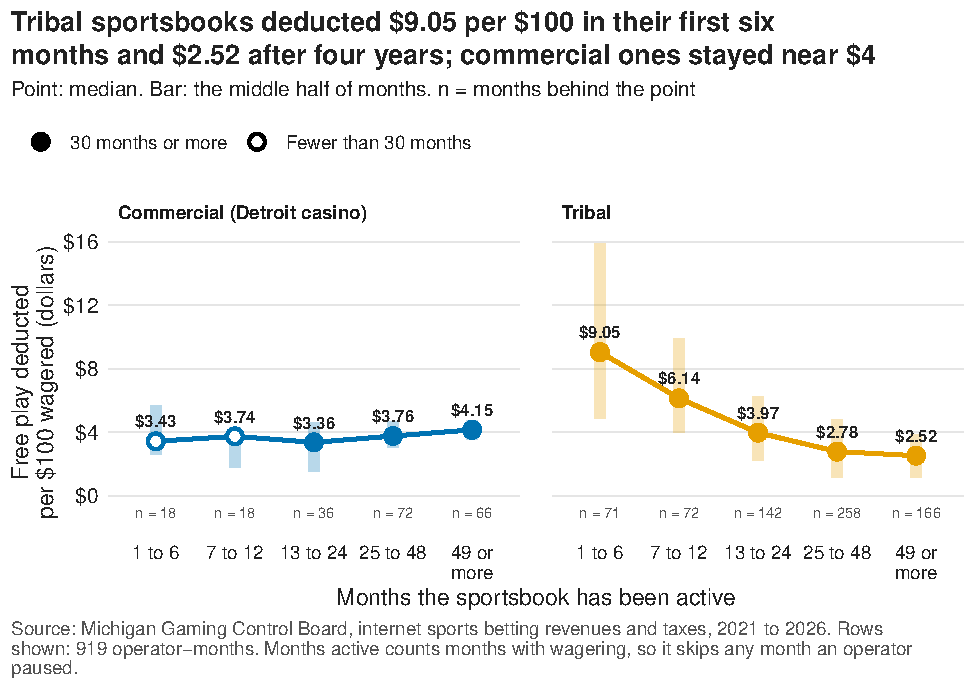
\includegraphics[width=0.92\linewidth]{figures/fig10_free_play_by_age_and_type.pdf}
\caption{Median free play per \$100 wagered by months active, within each operator type (sub-question 10). Source: Michigan Gaming Control Board; \V{fp_rows} sportsbook-months.}\label{fig:age}
\end{figure}

Taking all months together, the two operator types are close: a median of \$\V{com_median} for commercial sportsbooks (\V{com_months} months) and \$\V{tri_median} for tribal ones (\V{tri_months}). Tribal months are far more spread out, with a middle half from \$\V{tri_q1} to \$\V{tri_q3} against \$\V{com_q1} to \$\V{com_q3}. Size tells little: the correlation between free play per \$100 and the size of the month is \V{r_fp_size} across \V{fp_rows} months. Months under \$1 million wagered have the lowest median (\$\V{size_band1_median}, \V{size_band1_months} months) and the three larger size bands are nearly level (\$\V{size_band2_median}, \$\V{size_band3_median} and \$\V{size_band4_median}). I expected commercial sportsbooks and bigger months to show more free play.

\subsection*{How often is no tax paid, and by whom? (sub-questions 8 and 9)}

Tribal sportsbooks paid nothing to the State in \V{tri_notax_n} of \V{tri_rows} months (\V{tri_notax_pct}\%), commercial ones in \V{com_notax_n} of \V{com_rows} (\V{com_notax_pct}\%), as I expected. Figure~\ref{fig:notax} adds time. For tribal sportsbooks the share fell from \V{tri_2021_notax_pct}\% in 2021 (\V{tri_2021_notax_n} of \V{tri_2021_rows} months) to \V{tri_2026_notax_pct}\% in 2026 (\V{tri_2026_notax_n} of \V{tri_2026_rows}), with a bump back to \V{tri_2024_notax_pct}\% in 2024. For the commercial sportsbooks it swung: \V{com_2022_notax_round}\% in 2022, \V{com_2024_notax_pct}\% in 2024 (\V{com_2024_notax_n} of \V{com_2024_rows} months), \V{com_2025_notax_pct}\% in 2025 and \V{com_2026_notax_round}\% in 2026. The 2026 figures cover January to October. I expected the share to rise. Table~\ref{tab:notax} gives every count.

\begin{figure}[H]
\centering
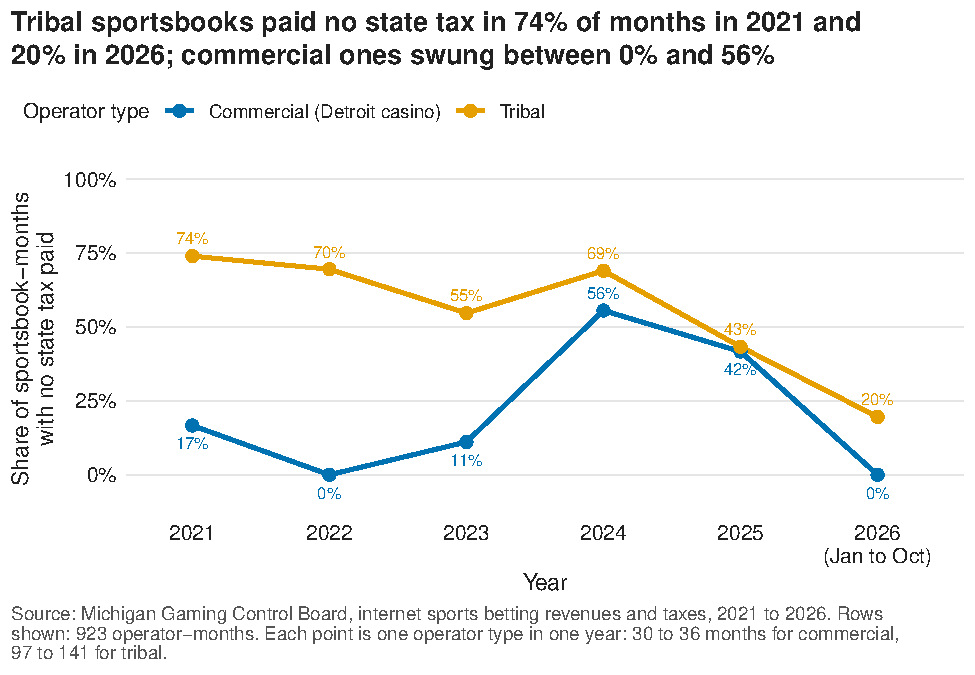
\includegraphics[width=0.92\linewidth]{figures/fig09_no_tax_by_year_and_type.pdf}
\caption{Share of sportsbook-months with no state tax paid, by year and operator type (sub-question 9). Source: Michigan Gaming Control Board; \V{rows_final} sportsbook-months.}\label{fig:notax}
\end{figure}

\begin{table}[H]
\centering\small
\caption{Months with no state tax paid, by year and operator type. Source: output/tables/eda\_09.}\label{tab:notax}
% Written by scripts/08_report_numbers.R from output/tables. Do not edit by hand.
\begin{tabular}{@{}llrrr@{}}
\toprule
Year & Operator type & Months & Months with no tax & Share with no tax (\%) \\
\midrule
2021 & commercial & 36 & 6 & 16.67 \\
2021 & tribal & 119 & 88 & 73.95 \\
2022 & commercial & 36 & 0 & 0.00 \\
2022 & tribal & 141 & 98 & 69.50 \\
2023 & commercial & 36 & 4 & 11.11 \\
2023 & tribal & 139 & 76 & 54.68 \\
2024 & commercial & 36 & 20 & 55.56 \\
2024 & tribal & 113 & 78 & 69.03 \\
2025 & commercial & 36 & 15 & 41.67 \\
2025 & tribal & 104 & 45 & 43.27 \\
2026 & commercial & 30 & 0 & 0.00 \\
2026 & tribal & 97 & 19 & 19.59 \\
\bottomrule
\end{tabular}

\end{table}

\subsection*{Do the unusual months change the picture? (sub-question 11)}

Leaving out the \V{lump_months} lump-deduction months and the \V{first_months} first months moves the overall median only from \$\V{fp_median} to \$\V{without_median} (\V{without_months} months left). Averages are another matter: the mean falls from \$\V{fp_mean} to \$\V{without_mean}, and the 2021 median from \$\V{yr_2021_median} to \$\V{without_2021}, because \V{lump_2021} of the lump months and \V{first_2021} of the first months fall in 2021. I expected no change at all. This report therefore uses medians, and the early-period numbers should be read with the flagged months in mind.

\subsection*{Which variables move together? (sub-question 12)}

Figure~\ref{fig:heatmap} is the correlation matrix of the two targets and the variables around them. Among things known before a month starts, free play per \$100 is most closely related to its own value the month before (\V{r_fp_prior}, \V{r_fp_prior_rows} months) and then to months active (\V{r_fp_months}). Paying no tax is most closely related to paying none the month before (\V{r_nt_prior}, \V{r_nt_prior_rows} months), to the size of the previous month (\V{r_nt_priorsize}) and to operator type (\V{r_nt_commercial} for commercial). My guess was that size would matter most for free play; its correlation is \V{r_fp_size}. Table~\ref{tab:corr} lists the correlations with each target.

The lump-deduction flag has the highest correlation with free play per \$100 of all (\V{r_fp_lump}), but it is built from the same month's deduction, so it is another version of the target and cannot be used to predict it. A correlation shows that two things move together in a straight line. It does not show that one causes the other.

\begin{figure}[H]
\centering
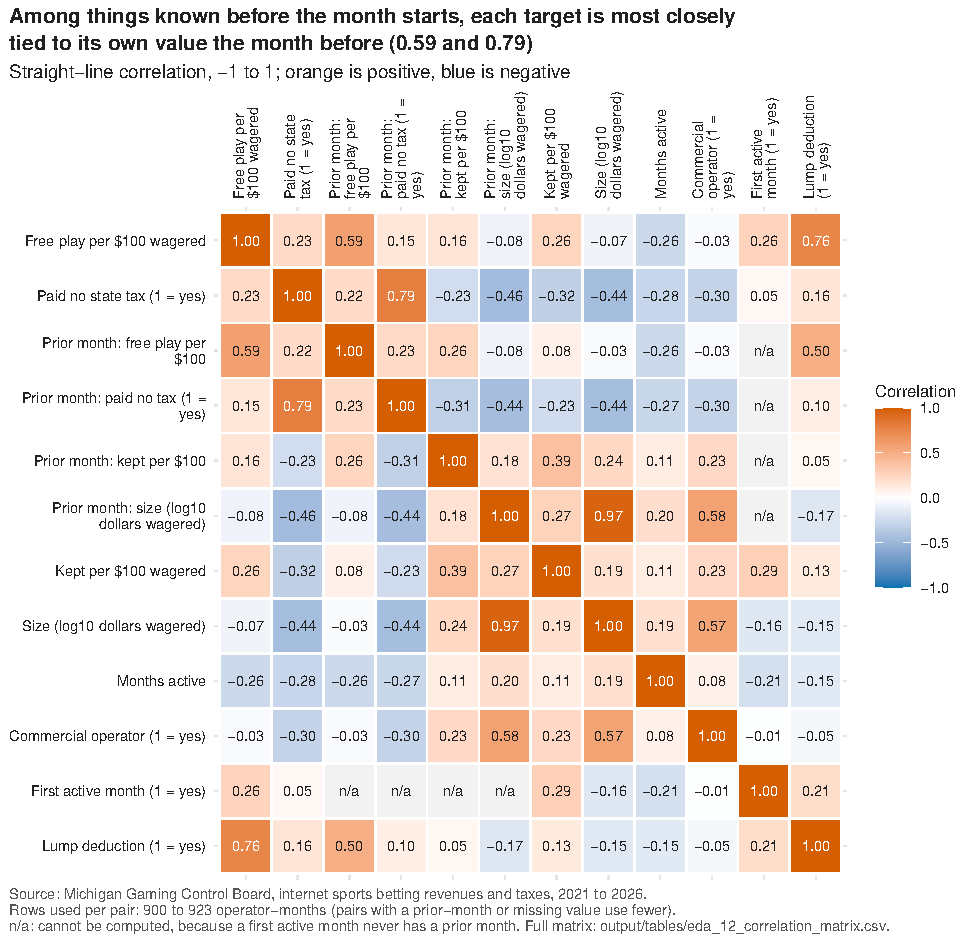
\includegraphics[width=\linewidth]{figures/fig12_correlation_heatmap.pdf}
\caption{Correlation matrix of the two targets and related variables (sub-question 12). Source: Michigan Gaming Control Board; \V{m1_rows} to \V{rows_final} sportsbook-months per pair.}\label{fig:heatmap}
\end{figure}

\begin{table}[H]
\centering\small
\caption{Correlation of each target with the variables known before the month starts. Source: output/tables/eda\_12c.}\label{tab:corr}
% Written by scripts/08_report_numbers.R from output/tables. Do not edit by hand.
\begin{tabular}{@{}p{0.27\linewidth}p{0.42\linewidth}rr@{}}
\toprule
Target & Variable known before the month starts & Correlation & Rows used \\
\midrule
Free play per \$100 wagered & Prior month: free play per \$100 & 0.59 & 900 \\
Free play per \$100 wagered & Months active & -0.26 & 919 \\
Free play per \$100 wagered & Year & -0.21 & 919 \\
Free play per \$100 wagered & Prior month: kept per \$100 & 0.16 & 902 \\
Free play per \$100 wagered & Prior month: paid no tax (1 = yes) & 0.15 & 903 \\
Free play per \$100 wagered & Prior month: size (log10 dollars wagered) & -0.08 & 903 \\
Free play per \$100 wagered & Month of the year (1 to 12) & -0.05 & 919 \\
Free play per \$100 wagered & Commercial operator (1 = yes) & -0.03 & 919 \\
Paid no state tax (1 = yes) & Prior month: paid no tax (1 = yes) & 0.79 & 906 \\
Paid no state tax (1 = yes) & Prior month: size (log10 dollars wagered) & -0.46 & 906 \\
Paid no state tax (1 = yes) & Commercial operator (1 = yes) & -0.30 & 923 \\
Paid no state tax (1 = yes) & Months active & -0.28 & 923 \\
Paid no state tax (1 = yes) & Prior month: kept per \$100 & -0.23 & 905 \\
Paid no state tax (1 = yes) & Year & -0.22 & 923 \\
Paid no state tax (1 = yes) & Prior month: free play per \$100 & 0.22 & 903 \\
Paid no state tax (1 = yes) & Month of the year (1 to 12) & -0.07 & 923 \\
\bottomrule
\end{tabular}

\end{table}

\section{Predictive models}\label{sec:models}

The predictive statement asks for two estimates at the start of a month. Both models here are ordinary linear regressions fitted to every row that has the needed values, and both are judged on those same rows. Each uses three predictors I chose from the correlation matrix, all known before the month starts. I recorded the direction I expected for each slope before either model was fitted.

\subsection*{The regression problem: free play per \$100 wagered}

\textbf{Target and predictors.} The target is free play deducted per \$100 wagered. The predictors are last month's free play per \$100 (the strongest correlation, \V{r_fp_prior}), the number of months the sportsbook has been active (\V{r_fp_months}), and operator type, which enters as 1 for a commercial sportsbook and 0 for a tribal one.

\textbf{Fitted equation.}
\begin{center}
free play per \$100 $=$ \V{m1_b0} $+$ \V{m1_b1} $\times$ (last month's free play per \$100) $-$ \V{m1_b2} $\times$ (months active) $+$ \V{m1_b3} $\times$ (commercial)
\end{center}

\begin{table}[H]
\centering\small
\caption{Model 1 estimates (\V{m1_rows} sportsbook-months). Source: output/tables/model1\_estimates.}\label{tab:m1}
% Written by scripts/08_report_numbers.R from output/tables. Do not edit by hand.
\begin{tabular}{@{}p{0.55\linewidth}rrr@{}}
\toprule
Term & Estimate & Standard error & p value \\
\midrule
Intercept (a tribal operator with every numeric predictor at zero) & 3.2356 & 0.4271 & under 0.001 \\
Prior month: free play per \$100 wagered & 0.4975 & 0.0243 & under 0.001 \\
Months the operator has been active & -0.0323 & 0.0099 & 0.001 \\
Commercial operator (1 = commercial, 0 = tribal) & 0.1308 & 0.4354 & 0.76 \\
\bottomrule
\end{tabular}

\end{table}

\textbf{What each slope means.} Table~\ref{tab:m1} gives the estimates. A sportsbook that deducted \$1 more of free play per \$100 last month tends to deduct about \V{m1_prior_cents} cents more per \$100 this month, holding months active and operator type fixed. I expected less, not more: heavy free play carries over from one month to the next. Each extra month a sportsbook has been active goes with about \V{m1_months_cents} cents less free play per \$100, or about \$\V{m1_months_year} less per year, holding the other two fixed. I expected it to go up; the result fits the launch pattern in Figure~\ref{fig:age}. A commercial sportsbook is predicted to deduct \$\V{m1_com_dollars} more per \$100 than a tribal one with the same history, but that estimate is small next to its standard error of \$\V{m1_com_se_dollars}, so the model does not tell the two types apart.

\textbf{Fit.} The model accounts for \V{m1_r2_pct}\% of the differences in free play per \$100 (R-squared \V{m1_r2}). Its typical miss, the root mean squared error, is \$\V{m1_rmse} per \$100, which is large beside a median of \$\V{fp_median}. A few months drive that figure. Figure~\ref{fig:m1a} and Figure~\ref{fig:m1b} show that \V{m1_within5_n} of the \V{m1_rows} predictions (\V{m1_within5_pct}\%) land within \$\V{def_within}, while \V{m1_above10} months came in more than \$\V{def_big_miss} above the prediction, the largest by \$\V{m1_largest_miss}; \V{m1_above10_lump} of those \V{m1_above10} are flagged lump-deduction months. \V{m1_left_out} rows were left out: \V{m1_no_prior} because the sportsbook has no month before it in the data and \V{m1_missing_value} because this month's or last month's free play value is blank.

\begin{figure}[H]
\centering
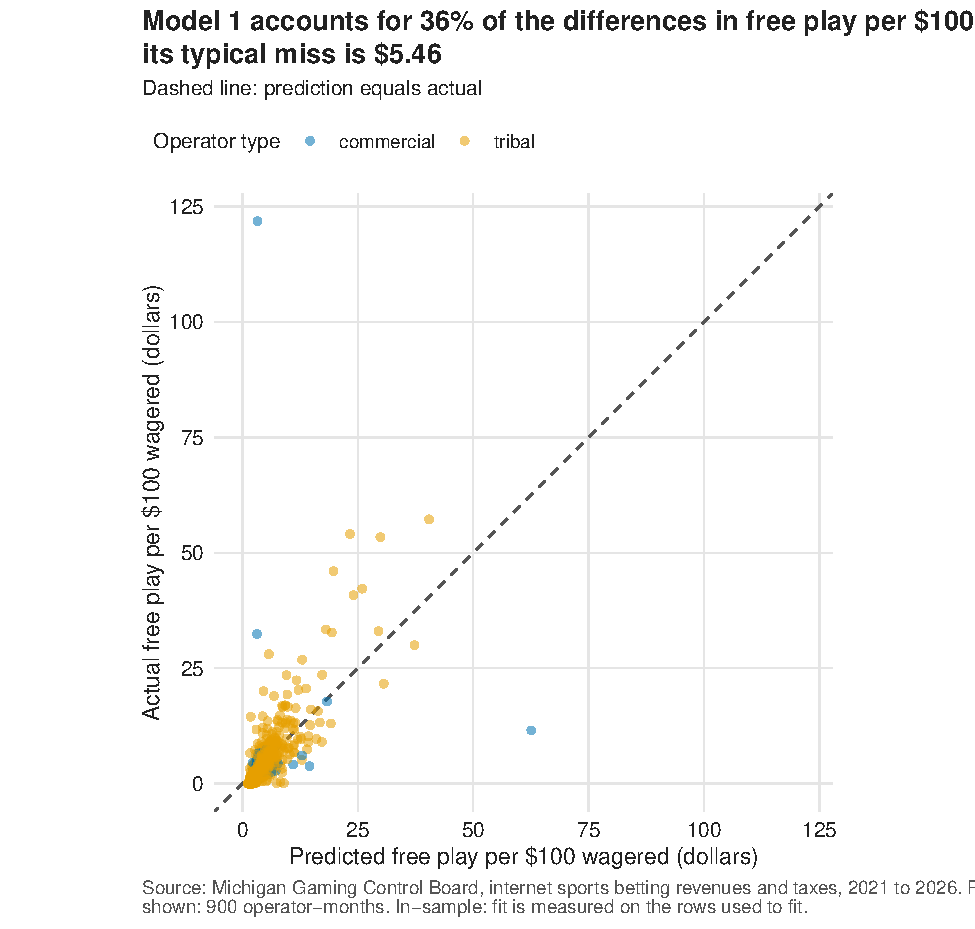
\includegraphics[width=0.74\linewidth]{figures/fig_m1_predicted_vs_actual.pdf}
\caption{Model 1: predicted against actual free play per \$100 wagered. Source: Michigan Gaming Control Board; \V{m1_rows} sportsbook-months, the rows used to fit.}\label{fig:m1a}
\end{figure}

\begin{figure}[H]
\centering
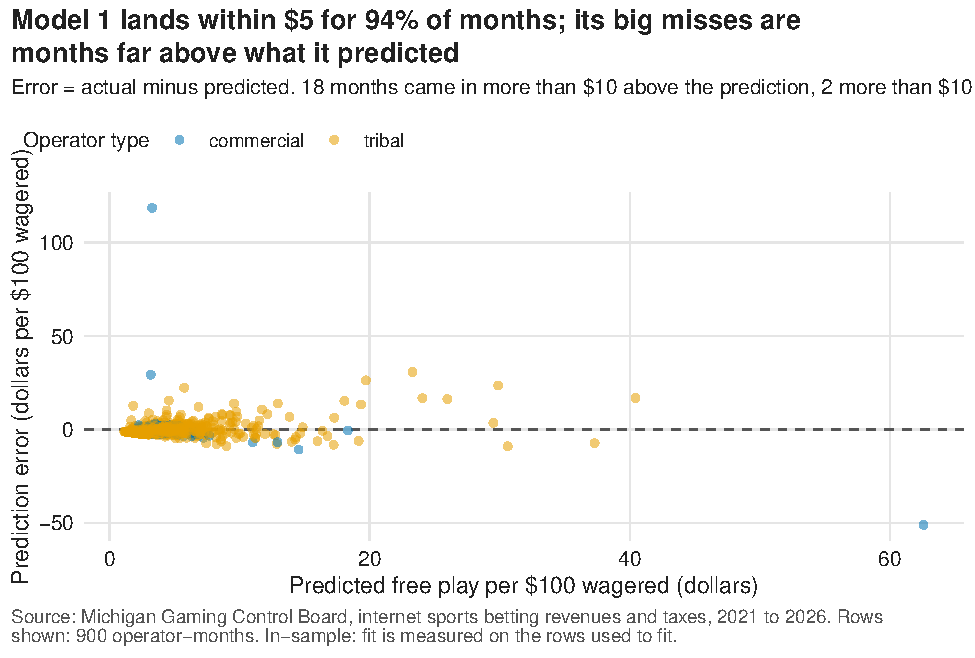
\includegraphics[width=0.92\linewidth]{figures/fig_m1_errors_vs_predicted.pdf}
\caption{Model 1: prediction errors against predicted values. Source: Michigan Gaming Control Board; \V{m1_rows} sportsbook-months, the rows used to fit.}\label{fig:m1b}
\end{figure}

\subsection*{The classification problem: paying no state tax}

\textbf{Target and predictors.} The target is 1 if the sportsbook paid no state tax or payment in the month and 0 if it paid something. A linear regression on a 0-and-1 target is a linear probability model, and its prediction is read as the probability of a yes. The predictors are whether the sportsbook paid no tax last month (\V{r_nt_prior}), the size of last month's wagering on a log scale, where one unit is a tenfold increase (\V{r_nt_priorsize}), and operator type.

\textbf{Fitted equation.}
\begin{center}
probability of no tax $=$ \V{m2_b0} $+$ \V{m2_b1} $\times$ (paid no tax last month) $-$ \V{m2_b2} $\times$ (log of last month's dollars wagered) $-$ \V{m2_b3} $\times$ (commercial)
\end{center}

\begin{table}[H]
\centering\small
\caption{Model 2 estimates (\V{m2_rows} sportsbook-months). Source: output/tables/model2\_estimates.}\label{tab:m2}
% Written by scripts/08_report_numbers.R from output/tables. Do not edit by hand.
\begin{tabular}{@{}>{\raggedright\arraybackslash}p{0.55\linewidth}rrr@{}}
\toprule
Term & Estimate & Standard error & p value \\
\midrule
Intercept (a tribal operator with every numeric predictor at zero) & 0.6532 & 0.1085 & under 0.001 \\
Prior month: paid no state tax (1 = yes, 0 = no) & 0.7353 & 0.0222 & under 0.001 \\
Prior month: size (log10 of dollars wagered) & -0.0771 & 0.0156 & under 0.001 \\
Commercial operator (1 = commercial, 0 = tribal) & -0.0084 & 0.0289 & 0.77 \\
\bottomrule
\end{tabular}

\end{table}

\textbf{What each slope means.} Table~\ref{tab:m2} gives the estimates. A sportsbook that paid no state tax last month has a predicted probability of paying none this month that is about \V{m2_prior_points} percentage points higher than one that paid, holding last month's size and operator type fixed. Each tenfold increase in last month's dollars wagered goes with a probability about \V{m2_size_points} percentage points lower, holding the other two fixed. Both are the directions I expected. A commercial sportsbook's predicted probability is \V{m2_com_points} percentage points lower than a tribal one's with the same history, with a standard error of \V{m2_com_se_points} points, so the model shows no difference between the types once last month's tax status and size are held fixed. The gap between the types in Section~\ref{sec:eda} (\V{tri_notax_pct}\% against \V{com_notax_pct}\%) goes with those two things in this model, not with type itself.

\textbf{Fit.} R-squared is \V{m2_r2}. Calling a prediction of \V{def_cutoff} or more a yes, Table~\ref{tab:class} shows the model is right for \V{m2_correct_n} of \V{m2_rows} months (\V{m2_correct_pct}\%). Always guessing the more common outcome, that tax was paid, would be right \V{m2_baseline_pct}\% of the time. The model misses in both directions: \V{m2_no_yes} months it called no-tax paid tax, and \V{m2_yes_no} months it called tax-paying paid none. \V{m2_outside} predictions (\V{m2_outside_pct}\%) fall outside 0 to 1, \V{m2_below0} below 0 and \V{m2_above1} above 1, with a largest value of \V{m2_max}; they are reported as they are (Figure~\ref{fig:m2}). \V{m2_left_out} rows were left out because the sportsbook has no month before it in the data.

\begin{table}[H]
\centering\small
\caption{Model 2: predicted against actual at the \V{def_cutoff} cutoff. Source: output/tables/model2\_classification\_table.}\label{tab:class}
% Written by scripts/08_report_numbers.R from output/tables. Do not edit by hand.
\begin{tabular}{@{}lrrr@{}}
\toprule
  & Predicted yes (0.5 or more) & Predicted no (under 0.5) & Total \\
\midrule
Actual: paid no tax (yes) & 394 & 43 & 437 \\
Actual: paid tax (no) & 50 & 419 & 469 \\
Total & 444 & 462 & 906 \\
\bottomrule
\end{tabular}

\end{table}

\begin{figure}[H]
\centering
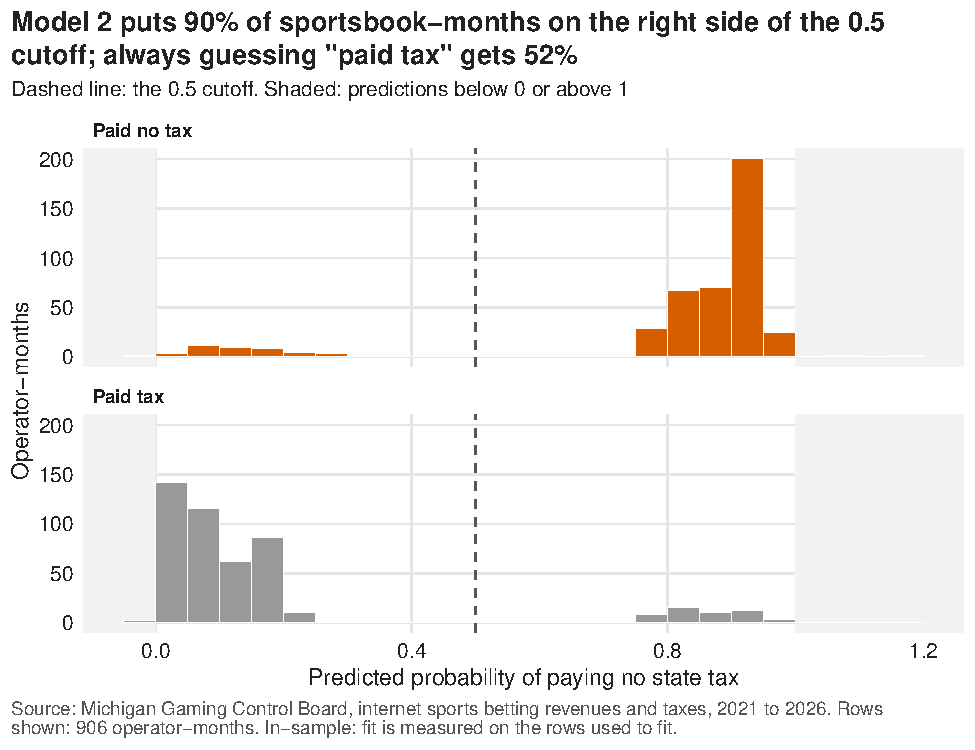
\includegraphics[width=0.92\linewidth]{figures/fig_m2_predicted_probability.pdf}
\caption{Model 2: predicted probability of paying no state tax, shown separately for months that did and did not. Source: Michigan Gaming Control Board; \V{m2_rows} sportsbook-months, the rows used to fit.}\label{fig:m2}
\end{figure}

\subsection*{Three cases}

Table~\ref{tab:cases} gives both predictions for three sportsbooks the Board might ask about. None of the values lies outside the range seen in the data. A large commercial sportsbook four years in is predicted to deduct \$\V{case1_m1} per \$100 and has a \V{case1_m2_pct}\% predicted probability of paying no tax. A small tribal sportsbook that paid no tax last month is predicted at \$\V{case2_m1} and \V{case2_m2_pct}\%. A tribal sportsbook in its fourth month with heavy free play is predicted at \$\V{case3_m1} and \V{case3_m2_pct}\%.

\begin{table}[H]
\centering
\caption{Scenario predictions from both models. Source: output/tables/model\_scenarios.}\label{tab:cases}
\resizebox{\linewidth}{!}{% Written by scripts/08_report_numbers.R from output/tables. Do not edit by hand.
\begin{tabular}{@{}p{0.27\linewidth}rrllrrrl@{}}
\toprule
Case & Free play last month (\$ per \$100) & Months active & Type & No tax last month & Wagered last month (\$) & Model 1 (\$ per \$100) & Model 2 (probability) & Beyond the data? \\
\midrule
1. Large commercial sportsbook, four years in, paid tax last month & 4.00 & 48 & commercial & no & 100,000,000 & 3.81 & 0.0278 & No \\
2. Small tribal sportsbook, five years in, paid no tax last month & 5.00 & 60 & tribal & yes & 1,500,000 & 3.78 & 0.9122 & No \\
3. Tribal sportsbook in its fourth month, heavy free play, paid no tax last month & 9.00 & 4 & tribal & yes & 3,000,000 & 7.58 & 0.8889 & No \\
\bottomrule
\end{tabular}
}
\end{table}

Both models describe association in these months, not cause. Fit was measured on the rows the models were fitted to, so these figures are a best case; on new months the models would probably do somewhat worse.

\section{Findings and recommendations}\label{sec:findings}

\subsection*{The answer to the descriptive statement}

\textbf{How much free play?} A typical sportsbook-month deducts \$\V{fp_median} for every \$100 wagered, and half of all months fall between \$\V{fp_q1} and \$\V{fp_q3}. \V{fp_pct_10plus}\% of months reach \$\V{def_fp_high} or more.

\textbf{How often is no tax paid?} In \V{notax_pct}\% of sportsbook-months, and far more often for tribal operators (\V{tri_notax_pct}\%) than for commercial ones (\V{com_notax_pct}\%).

\textbf{Who leans hardest on free play?} Not the biggest brands. FanDuel, DraftKings and BetMGM take \V{share_top3_total}\% of the wagering and sit near the median. The highest medians belong to two smaller tribal sportsbooks, at \$\V{op_lvd_median} and \$\V{op_hannahville_median} per \$100.

\textbf{Is it fading?} For tribal sportsbooks, yes: free play per \$100 went from \$\V{age_tri_b1_median} in the first six months to \$\V{age_tri_b5_median} after four years, and the share of months with no tax from \V{tri_2021_notax_round}\% in 2021 to \V{tri_2026_notax_round}\% in 2026. For commercial sportsbooks the median stayed between \$\V{age_com_min} and \$\V{age_com_max} at every age, and most of their no-tax months came in 2024 and 2025.

\subsection*{What the models add}

Both targets carry over from one month to the next. That makes the no-tax outcome easy to anticipate: knowing last month's tax status and size is enough to call \V{m2_correct_pct}\% of months correctly on the data in hand. It does not make free play per \$100 easy to anticipate. The first model's typical miss of \$\V{m1_rmse} is larger than the median itself, and \V{m1_above10_lump} of its \V{m1_above10} largest misses are lump-deduction months, which nothing in the model points to beforehand.

\subsection*{What the Board should do or look at next}

\begin{enumerate}
\item \textbf{Order the review of free-play claims by last month's result.} Start each month with the sportsbooks that paid no tax the month before and are small. That is where the second model puts the highest probability of another month with no tax.
\item \textbf{Track lump deductions as their own item.} \V{lump_months} months hold deductions larger than \V{def_lump_share} of the dollars wagered. With them the average is \$\V{fp_mean} per \$100; without them it is \$\V{without_lump_mean}. Knowing which months of promotion each lump belongs to would remove most of that noise.
\item \textbf{Watch launches and relaunches.} Tribal sportsbooks deducted \$\V{age_tri_b1_median} per \$100 in their first six months. A new operator, or an existing license moving to a new brand, is the point at which heavy free play should be expected.
\item \textbf{Look into the commercial no-tax months of 2024 and 2025.} \V{com_2024_notax_n} of \V{com_2024_rows} commercial months in 2024 and \V{com_2025_notax_n} of \V{com_2025_rows} in 2025 had no tax paid, after \V{com_2021_notax_n}, \V{com_2022_notax_n} and \V{com_2023_notax_n} in the three years before. This report describes that change; it does not explain it.
\item \textbf{Do not set a cap from these numbers alone.} They show what was deducted, not what would have happened to wagering, promotions or tax under a cap.
\end{enumerate}

\section{Limitations}\label{sec:limits}

\textbf{Coverage.} The data cover internet sports betting in Michigan only. Retail sports betting and internet casino games are reported separately and are not here, although the same companies run them. The last year stops in October 2026, so 2026 is not a full year.

\textbf{Who is missing.} There are no bettors in these data. One row is a sportsbook's month, so the report cannot say who received free bets, how they were used, or whether anyone was harmed. Three operators stopped offering internet sports betting during the period, and their later months are absent.

\textbf{Measurement.} Free play is not published. It is taken as gross receipts minus adjusted gross receipts, the deduction the law allows, in the month it was claimed. An operator can claim it late, which is why \V{lump_months} months are flagged. The publisher does not define ``Total Handle''; if it includes wagers placed with free bets, the dollars wagered by heavy promoters are overstated. The figures are as reported by operators, and the workbooks say not all have been audited. Brand names are each operator's latest platform, not a record of which brand ran in each month.

\textbf{Small groups and extreme values.} Commercial results rest on \V{n_commercial} sportsbooks, and some groups are small: the first two commercial age bands hold \V{age_com_b1_months} months each. Medians are used throughout because a few very large months move the averages.

\textbf{What description cannot establish.} Every result here is an association. The report cannot say that free play causes a month with no tax, that age causes free play to fall (\V{first_2021} of the \V{first_months} operators started in 2021, so age and calendar time can hardly be separated), or what a cap would do. Other explanations for each main finding, and a check that would tell them apart, are listed in the repository (documentation/eda\_alternatives.md); none of those checks has been run.

\textbf{The models.} Each model was judged on the rows it was fitted to. Nothing was held back to test them, so their fit is a best case. A linear probability model can predict below 0 or above 1, and this one did \V{m2_outside} times. The rows of one sportsbook in neighboring months are not independent, which the standard errors do not allow for.

\textbf{Provenance.} Three fields of the provenance record (the version date, the citation form the publisher prefers, and a second reading of the quoted legal text) were still open when this draft was written.

\section{Next steps}\label{sec:next}

\textbf{Testing and improving the predictions.} The honest test of a forecast is on months the model has not seen: fit on the earlier years, predict the latest one, and compare. That, and methods built for a yes-or-no target that cannot stray outside 0 to 1, are the subject of BUAN 381. Predictors worth trying there include the season of the year, a sportsbook's own average over the past year in place of a single month, and whether a lump deduction was taken recently.

\textbf{The prescriptive statement.} The decision is the cap on the monthly free-play deduction, as a percent of gross sports betting receipts, that the Board should recommend to the Legislature. The objective is to collect the most state and city tax. The constraints are one cap for every operator, and no cap below the share of gross receipts that the median sportsbook-month actually deducted.

Solving it needs things these data do not have: free play issued in each month and not only claimed; how wagering and promotions respond when the deduction is limited; and how each dollar of tax is divided between the State and the city of Detroit.


\bibliographystyle{plain}
\bibliography{references}

\appendix
\section{Codebook}

One row per variable in the cleaned data (\V{rows_final} rows, \V{n_columns} columns). The complete codebook, with allowed values, observed ranges, where each variable comes from and how it was transformed, is \texttt{documentation/codebook.md} in the repository.

{\footnotesize
% Written by scripts/08_report_numbers.R. Do not edit by hand.
\begin{longtable}{@{}>{\raggedright\arraybackslash}p{0.22\linewidth}>{\raggedright\arraybackslash}p{0.33\linewidth}>{\raggedright\arraybackslash}p{0.10\linewidth}>{\raggedright\arraybackslash}p{0.13\linewidth}>{\raggedright\arraybackslash}p{0.10\linewidth}@{}}
\toprule
\textbf{Name} & \textbf{Label} & \textbf{Type} & \textbf{Units} & \textbf{Missing} \\
\midrule
\endhead
\bottomrule
\endfoot
operator & Licensed internet sports betting operator (the licensee) & Category & none & 0.0\% (0 of 923) \\
operator\_short & Short operator name for figures & Category & none & 0.0\% (0 of 923) \\
operator\_type & Whether the operator is a commercial Detroit casino or a tribal operator & Category & none & 0.0\% (0 of 923) \\
casino\_name & Casino or casinos tied to the operator's license & Text & none & 0.0\% (0 of 923) \\
platform\_as\_listed & Platform provider (the betting brand) as printed on that year's sheet & Text & none & 0.0\% (0 of 923) \\
platform\_latest & The operator's platform provider as printed on its most recent sheet & Text & none & 0.0\% (0 of 923) \\
launch\_date & Initial date of operation launch & Date & date & 0.0\% (0 of 923) \\
year & Calendar year of the reporting month & Whole number & year & 0.0\% (0 of 923) \\
month & Calendar month of the reporting month & Whole number & month number & 0.0\% (0 of 923) \\
month\_name & Name of the reporting month & Category & none & 0.0\% (0 of 923) \\
month\_date & First day of the reporting month & Date & date & 0.0\% (0 of 923) \\
handle & Total dollars wagered online with the operator in the month & Number & US dollars & 0.0\% (0 of 923) \\
gross\_receipts & Gross sports betting receipts: all sums wagered with the operator, less winnings, refunded or voided wagers, and uncollectible amounts & Number & US dollars & 0.0\% (0 of 923) \\
adjusted\_gross\_receipts & Adjusted gross sports betting receipts: gross receipts less the deduction for free play & Number & US dollars & 0.0\% (0 of 923) \\
state\_tax\_or\_payment & Tax (commercial operators) or payment (tribal operators) to the State for the month, as reported & Number & US dollars & 0.0\% (0 of 923) \\
free\_play\_deduction & Free play deducted in the month it was claimed & Number & US dollars & 0.2\% (2 of 923) \\
free\_play\_per\_100 & Free play deducted per \$100 wagered & Number & dollars per \$100 wagered (percent of handle) & 0.4\% (4 of 923) \\
kept\_per\_100 & Dollars the operator kept per \$100 wagered, before free play is deducted & Number & dollars per \$100 wagered (percent of handle) & 0.2\% (2 of 923) \\
paid\_no\_tax & Whether the operator paid no state tax or payment for the month & Category (0 or 1) & none & 0.0\% (0 of 923) \\
log10\_handle & Size of the month's wagering: base-10 logarithm of handle & Number & log10 of US dollars & 0.0\% (0 of 923) \\
months\_active & Count of months with wagering for this operator up to and including this one & Whole number & months & 0.0\% (0 of 923) \\
first\_active\_month & Whether this is the operator's first month with wagering & Category (0 or 1) & none & 0.0\% (0 of 923) \\
lump\_deduction & Whether the free play deducted is more than a quarter of the month's handle & Category (0 or 1) & none & 0.0\% (0 of 923) \\
prior\_free\_play\_per\_100 & The same operator's free play per \$100 wagered in the previous calendar month & Number & dollars per \$100 wagered & 2.2\% (20 of 923) \\
prior\_kept\_per\_100 & The same operator's dollars kept per \$100 wagered in the previous calendar month & Number & dollars per \$100 wagered & 2.0\% (18 of 923) \\
prior\_log10\_handle & The same operator's log10 of handle in the previous calendar month & Number & log10 of US dollars & 1.8\% (17 of 923) \\
prior\_paid\_no\_tax & Whether the same operator paid no state tax or payment in the previous calendar month & Category (0 or 1) & none & 1.8\% (17 of 923) \\
source\_file & The raw workbook the row was read from & Category & none & 0.0\% (0 of 923) \\
\end{longtable}

}

\section{Wrangling log}

Every cleaning step in the order it ran, with the reason and the row count before and after. Steps 16a and 16b are the two parts of step 16.

{\footnotesize
% Written by scripts/08_report_numbers.R. Do not edit by hand.
\begin{longtable}{@{}>{\raggedright\arraybackslash}p{0.05\linewidth}>{\raggedright\arraybackslash}p{0.38\linewidth}>{\raggedright\arraybackslash}p{0.31\linewidth}rr@{}}
\toprule
\textbf{Step} & \textbf{What changed} & \textbf{Why} & \textbf{Before} & \textbf{After} \\
\midrule
\endhead
\bottomrule
\endfoot
1 & Reshaped the wide workbooks to one row per operator per month. No value changed. & One row must be one operator in one month. & 1,956 & 1,956 \\
2 & Kept each year's copy from the newest workbook that carries it; removed the duplicate copy. & Every year except 2026 appears in two workbooks; the copies agree in every cell where both hold a number. & 1,956 & 1,068 \\
3 & Dropped months that are blank for every operator (December 2026, November 2026). & They have not been reported yet, so they are not observations. & 1,068 & 1,038 \\
4 & Dropped operator-months with no wagering: Total Handle zero (96) or blank (18). Receipts and tax are zero or blank in all of them. & The question is about sportsbooks that are operating; these are months before launch, after stopping, or paused. & 1,038 & 924 \\
5 & Dropped the row with a negative Total Handle (Little Traverse Bay Bands of Odawa Indians, August 2023: -1,419.34). & A closing correction after the operator stopped, not a month of betting. & 924 & 923 \\
10 & Removed typed footnote markers from operator names (19 labels became 15 names) and added a short name for figures. & One operator needs one name. & 923 & 923 \\
11 & Kept the platform provider (brand) as printed on each year's sheet and added each operator's latest label as a second column. & Brand labels change across years; the operator is the stable key. & 923 & 923 \\
12 & Created operator type from the label of the tax column: commercial (210 rows), tribal (713 rows). & Operator type is not a column in the file. & 923 & 923 \\
13 & Converted the launch date from a spreadsheet day number in text to a date (one cell held text and reads as the same date as its other form). & Wrong type in the file. & 923 & 923 \\
7 & No change: 50 months with negative gross receipts kept as reported. & A sportsbook can pay out more than it takes in a month. & 923 & 923 \\
15 & No change: tax or payment kept as reported, including 232 months with positive adjusted receipts and zero tax. & The reported figure is what was paid; it defines the yes-or-no target. & 923 & 923 \\
16a & Created: month\_date, free\_play\_deduction (gross minus adjusted receipts), free\_play\_per\_100, kept\_per\_100, paid\_no\_tax, log10\_handle, months\_active. & Needed by the problem statements; each is defined in the codebook. & 923 & 923 \\
9 & Added the flag lump\_deduction = 1 where the deduction is more than a quarter of that month's handle. No value changed. & Free play can be claimed in a later month as a lump; the flag lets findings be checked with and without those months. & 923 & 923 \\
14 & Added the flag first\_active\_month = 1 for each operator's first month with wagering. No value changed. & First months are partial (January 2021 starts on the 22nd). & 923 & 923 \\
8 & Kept the rows; set free\_play\_deduction and free\_play\_per\_100 to missing where adjusted receipts exceed gross receipts. & A negative amount is not free play and the file does not explain it. & 923 & 923 \\
6 & Kept the rows; set free\_play\_per\_100 and kept\_per\_100 to missing where Total Handle is under \$10,000. & Ratios on a few hundred dollars are not meaningful. & 923 & 923 \\
16b & Created prior-month versions (prior\_free\_play\_per\_100, prior\_kept\_per\_100, prior\_log10\_handle, prior\_paid\_no\_tax), filled only when the operator's previous calendar month is in the data (906 of 923 rows). & Things known at the start of a month, for the predictive statement. & 923 & 923 \\
17 & Gave columns plain lower-case names and fixed their order (28 columns). Dollar amounts are kept exactly as published, with no rounding. & Clear names; no value changed. & 923 & 923 \\
\end{longtable}

}

\section{AI-use statement}

% This statement is Brennan's. The paragraphs below are a factual draft by the AI assistant,
% taken from the project's prompt log and decision log. Brennan revises it at his final pass
% so that it says, truthfully, what he wrote himself.

This project was carried out with an AI coding assistant, Claude Code (model Claude Fable 5.2), working in the project folder under my direction. Every prompt and its result is recorded in \texttt{documentation/prompt\_log.md}, and every decision with who made it in \texttt{documentation/process/decision\_log.md}.

\textbf{What the assistant did.} It wrote and ran all of the R code; audited the raw data; proposed the cleaning plan, the exploration sub-questions and the candidate predictors; built the tables, figures, both reports and the logs; and proofread by listing problems.

\textbf{What I did.} I chose the topic, the decision-maker and the two targets. I downloaded the six workbooks myself. I decided every one of the \V{cleaning_decisions} cleaning steps. I chose what I expected for each sub-question and for each model slope before the analysis ran, by picking from options the assistant offered. I chose the predictors.

\textbf{The wording of this report.} \ifdraft The text of this draft was written by the AI assistant and is labeled as its draft in the repository. I have not yet revised it. \else [Brennan: state here which parts you rewrote and which you kept as drafted.] \fi

\textbf{Checks on the assistant's work.} Each data step has a stated expected count that was compared with the result; \V{tests_run} tests guard the cleaned data; \V{hand_equal} of \V{hand_checks} hand-worked predictions equal the script's; and every number in this report is read from a results file by a script, not typed.


\end{document}
